%%%%%%%%%%%%%%%%%%%%%%%%%%%%%%%%%%%%%%%%%
% Awesome Cover Letter
% XeLaTeX Template
% Version 1.3 (30/3/2020)
%
% This template has been downloaded from:
% http://www.LaTeXTemplates.com
%
% Original authors:
% Claud D. Park (posquit0.bj@gmail.com)
% Lars Richter (mail@ayeks.de)
% With modifications by:
% Vel (vel@latextemplates.com)
%
% License:
% CC BY-NC-SA 3.0 (http://creativecommons.org/licenses/by-nc-sa/3.0/)
%
% Important note:
% This template must be compiled with XeLaTeX, the below lines will ensure this
%!TEX TS-program = xelatex
%!TEX encoding = UTF-8 Unicode
%
%%%%%%%%%%%%%%%%%%%%%%%%%%%%%%%%%%%%%%%%%

%----------------------------------------------------------------------------------------
%	PACKAGES AND OTHER DOCUMENT CONFIGURATIONS
%----------------------------------------------------------------------------------------

\documentclass[11pt, a4paper]{awesome-cv} % A4 paper size by default, use 'letterpaper' for US letter
\usepackage{pdfpages}

\geometry{left=2cm, top=1.5cm, right=2cm, bottom=2cm, footskip=.5cm} % Configure page margins with geometry
 
\fontdir[fonts/] % Specify the location of the included fonts

% Color for highlights
\colorlet{awesome}{awesome-skyblue} % Default colors include: awesome-emerald, awesome-skyblue, awesome-red, awesome-pink, awesome-orange, awesome-nephritis, awesome-concrete, awesome-darknight
%\definecolor{awesome}{HTML}{CA63A8} % Uncomment if you would like to specify your own color

% Colors for text - uncomment and modify
%\definecolor{darktext}{HTML}{414141}
%\definecolor{text}{HTML}{414141}
%\definecolor{graytext}{HTML}{414141}
%\definecolor{lighttext}{HTML}{414141}

\renewcommand{\acvHeaderSocialSep}{\quad\textbar\quad} % If you would like to change the social information separator from a pipe (|) to something else

%----------------------------------------------------------------------------------------
%	PERSONAL INFORMATION
%	Comment any of the lines below if they are not required
%----------------------------------------------------------------------------------------

\name{}{Alireza Zakeri}
%\address{246-1002, Gwangmyeongmayrouge Apt. 86, Cheongna lime-ro, Seo-gu, Incheon-si, 404-180, Rep. of KOREA}
\mobile{+989125071633}

\email{Alireza\_zak@yahoo.com}
%\homepage{www.posquit0.com}
\github{Alirezazak}
\linkedin{Alireza-Zakeri-a5b40587}{Alireza Zakeri}
\skype{rezaii995}
%\stackoverflow{SOid}{SOname}
%\twitter{@twit}
%\reddit{reddit account}
%\xing{xing name}
%\extrainfo{test} % Other text you want to include on this line

\position{Embedded System Developer Engineer{\enskip\cdotp\enskip}Hardware Designer on FPGAs} % Your expertise/fields
%\quote{``Make the change that you want to see in the world."} % A quote or statement

%----------------------------------------------------------------------------------------
%	RECIPIENT/POSITION/LETTER INFORMATION
%	All of the below lines must be filled out
%----------------------------------------------------------------------------------------

%\recipient{Company Recruitment Team}{Initech Inc.\\4120 Freidrich Ln.\\Austin, TX 78744} % The company being applied to

\letterdate{\today} % The date on the letter, default is the date of compilation

\lettertitle{Job Application for Middle Manager} % The title of the letter

\letteropening{Dear Mr./Ms./Dr. LastName,} % How the letter is opened

\letterclosing{Sincerely,} % How the letter is closed

\letterenclosure[Attached]{Curriculum Vitae} % Any enclosures with the letter

\makecvfooter{\today}{Alireza Zakeri~~~·~~~Cover Letter}{} % Specify the letter footer with 3 arguments: (<left>, <center>, <right>), leave any of these blank if they are not needed
  
%----------------------------------------------------------------------------------------

\begin{document}

\makecvheader[R] % Print the header

\makelettertitle[R] % Print the title

%----------------------------------------------------------------------------------------
%	LETTER CONTENT
%----------------------------------------------------------------------------------------

\begin{cvletter}

%------------------------------------------------

\lettersection{About Me}

I'm a qualified embedded system developer engineer with 4+ years of experience particularly in HDL circuit design and real-time processor-based systems development. I have practical experience in the customization and configuration of Linux kernel, U-Boot, and RTOS on Xilinx and TI cutting-edge SoCs (Zynq, ZynqMP, Keystone I, and II). Also, I'm an expert in developing hardware on high-tech Xilinx FPGAs (7 Series and UltraScale). In addition, I'm familiar with many low-rate and high-rate protocols (I2C, SPI, UART, etc) and microcontrollers (Atmel and STM32) programming.

I've graduated with a master's degree in electronics from Iran University of Science and Technology (IUST) which is one of the top-ranked universities of Iran.

Eager to collaborate and work in a team, interested in devising a better problem-solving method for challenging tasks, and learning new technologies and tools if the need arises.

%------------------------------------------------

\lettersection{Why Initech?}

Prepared by experienced English teachers, the texts, articles and conversations are brief and appropriate to your level of proficiency. Take the multiple-choice quiz following each text, and you'll get the results immediately. You will feel both challenged and accomplished! You can even download (as PDF) and print the texts and exercises. It's enjoyable, fun and free. Good luck!

%------------------------------------------------

\lettersection{Why Me?}

English texts for beginners to practice reading and comprehension online and for free. Practicing your comprehension of written English will both improve your vocabulary and understanding of grammar and word order. The texts below are designed to help you develop while giving you an instant evaluation of your progress.

%------------------------------------------------

\end{cvletter}

%----------------------------------------------------------------------------------------

\makeletterclosing % Print the signature and enclosures

%----------------------------------------------------------------------------------------
\newpage % Force a new page for looks
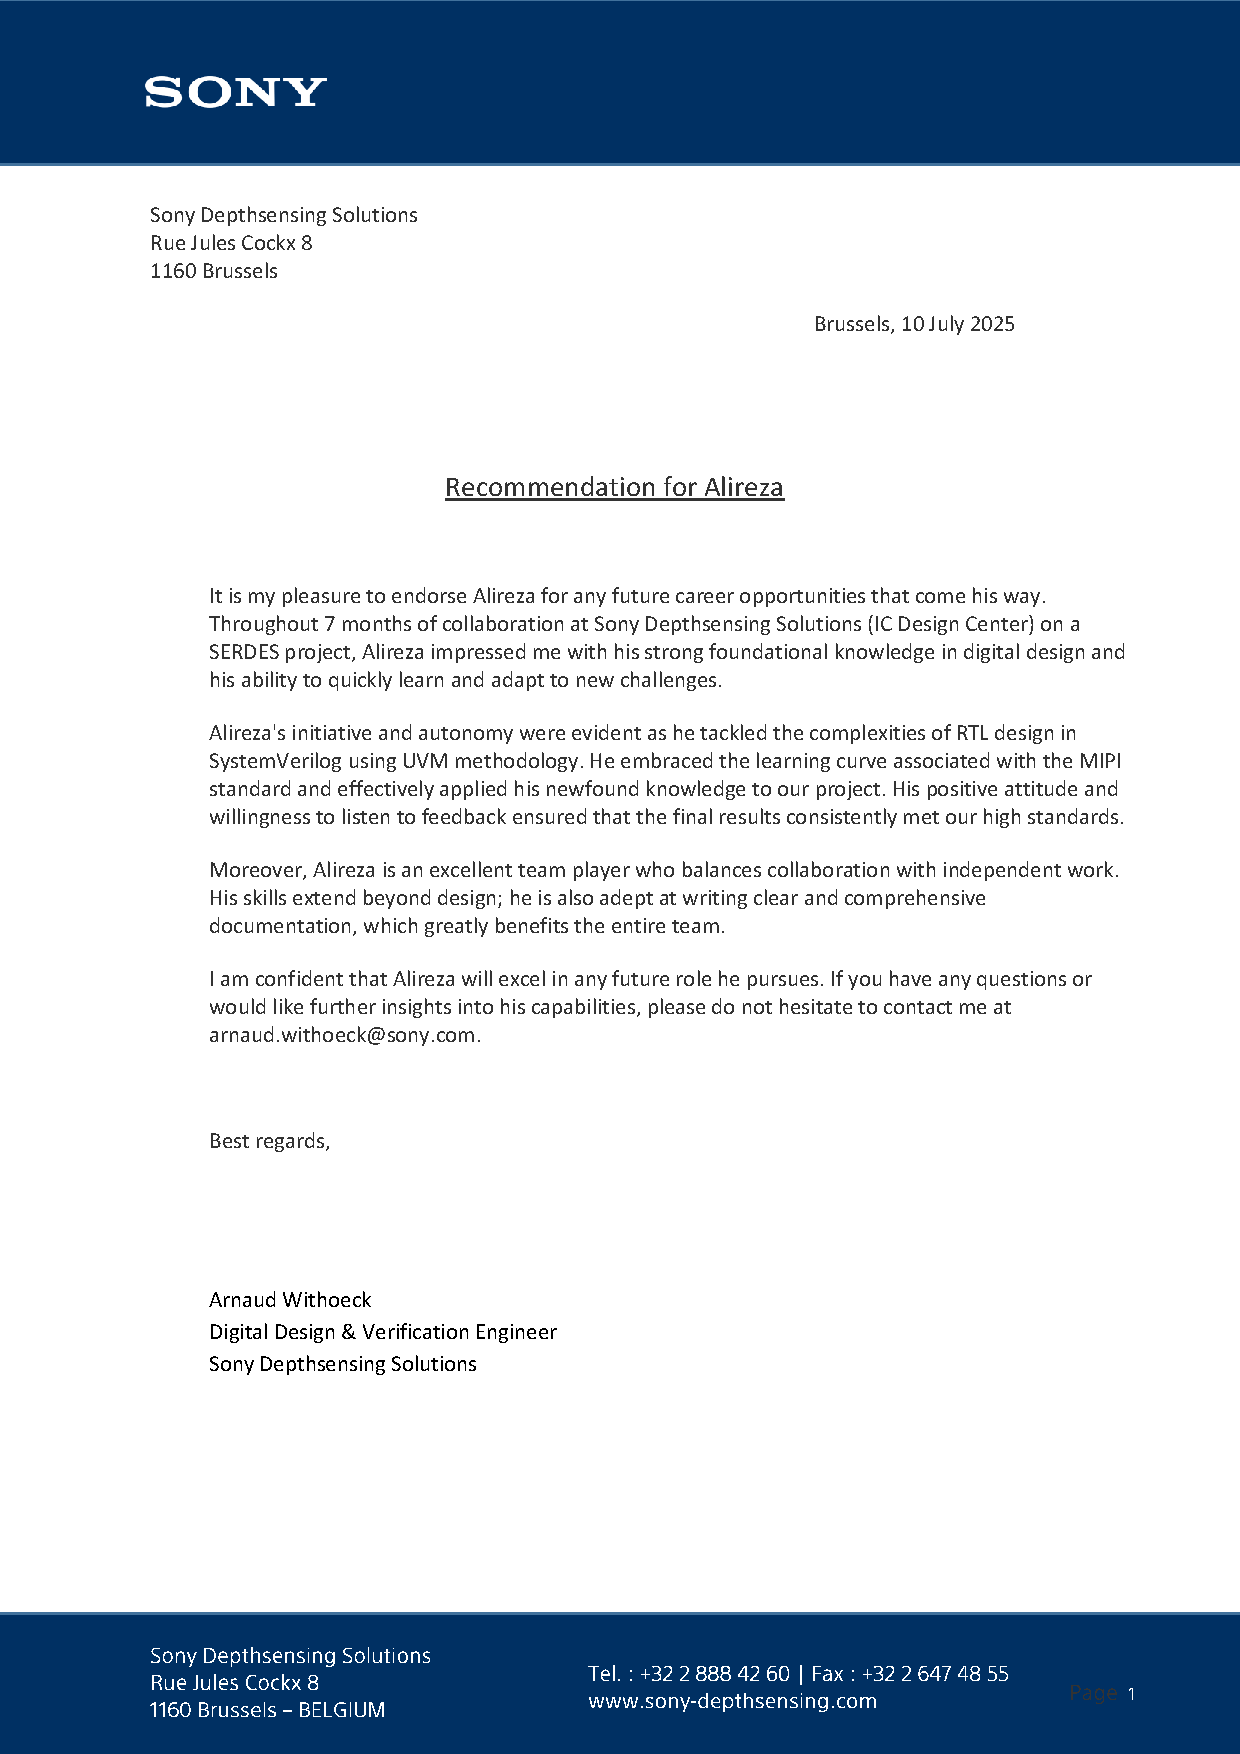
\includepdf[pages=-]{cv-sections/Sony.pdf}
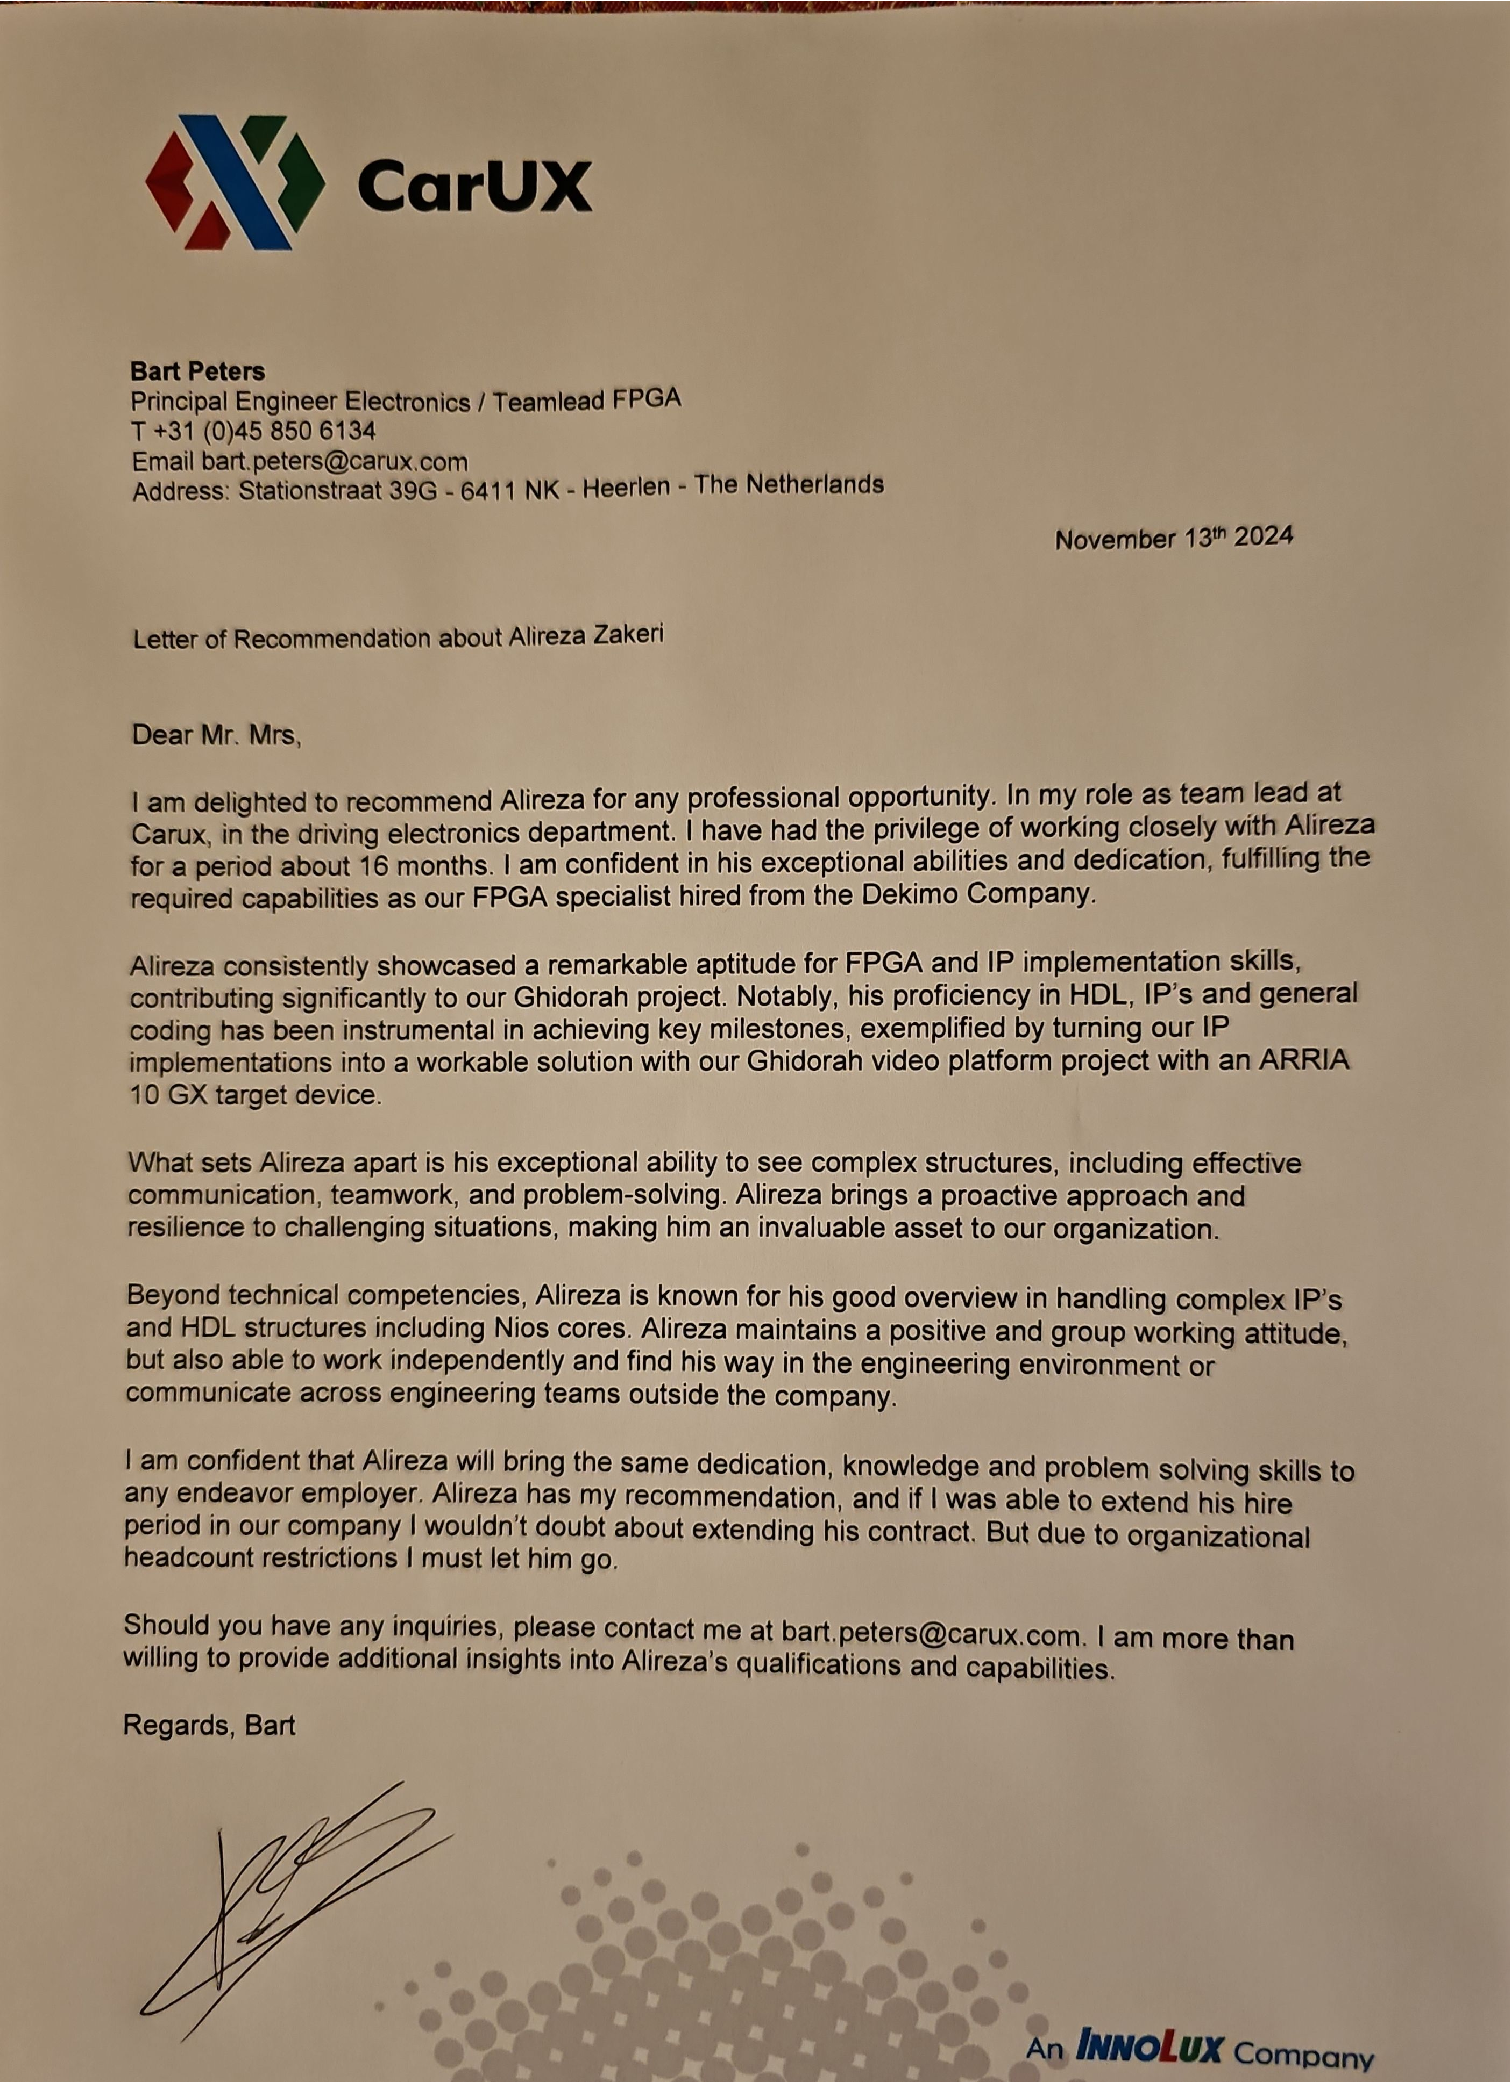
\includepdf[pages=-]{cv-sections/carux.pdf}

\end{document}
